% IPCCC 2026 — 5D H-NGAC manuscript
% Numbers: docs/canonical-context.md .
% Build: pdflatex main && bibtex main && pdflatex main && pdflatex main
\documentclass[conference]{IEEEtran}
\usepackage{amsmath,amssymb}
\usepackage{booktabs}
\usepackage{graphicx}
\usepackage{url}
\usepackage[table]{xcolor}
\graphicspath{{figures/}}

% hyperref LAST, after every other package. hidelinks keeps Section/Table/Figure
% and citation numbers clickable without printing them in a box or a color, which
% matters here for two reasons: IEEE wants a print-clean PDF, and this draft
% already uses red for the \new{} review markup, so colored links would collide.
\usepackage[hidelinks,breaklinks]{hyperref}


% TO TURN THE MARKING OFF FOR SUBMISSION: change the \new definition below to
%     \newcommand{\new}[1]{#1}
% and change \newcolor to a no-op:
%     \newcommand{\newcolor}{}
% Nothing else needs touching, and the two commands must stay defined because
% they are used inside table bodies where \textcolor cannot span rows.
% Score ramp for the related-work rubric. One pastel per score 0..5, stepped so
% grayscale luminance falls monotonically 91.6% -> 59.0% as the score rises. That
% ordering is what makes the table readable in black-and-white print and under
% red-green color blindness: magnitude is carried by lightness, and hue only
% reinforces it. Black text keeps >12.8:1 contrast on every step.
% \sco{n} paints a cell with the tint for score n and prints n.
\definecolor{sc0}{HTML}{F7F5F3}
\definecolor{sc1}{HTML}{FCEDE1}
\definecolor{sc2}{HTML}{FBE5C8}
\definecolor{sc3}{HTML}{EEE6A2}
\definecolor{sc4}{HTML}{D2E4A0}
\definecolor{sc5}{HTML}{A6D6A6}
\newcommand{\sco}[1]{\cellcolor{sc#1}#1}
\newcommand{\scob}[1]{\cellcolor{sc#1}\textbf{#1}}
\definecolor{hkred}{rgb}{0.72,0.06,0.06}
\newcommand{\new}[1]{\textcolor{hkred}{#1}}
\newcommand{\newcolor}{\color{hkred}}

\begin{document}

% OLD --- Security Dimensionality at Zero Time Cost: A Provenance-Aware 5D H-NGAC Authorization Primitive on FPGA
% Two lines, and 15 characters SHORTER than the Low-Latency version, so the space
% constraint is met without claiming low latency (Sec. VI-G concedes the CPU wins
% the mean by ~19x). Revert to the Low-Latency line if you disagree.
\title{Authenticated but Unauthorized: Bounded-Latency 5D H-NGAC for Real-Time Robotics}


\author{
    \IEEEauthorblockN{Hassan Karim\IEEEauthorrefmark{1},
    Md Omar Faruque\IEEEauthorrefmark{2},
    Abdel-Hameed A.\ Badawy\IEEEauthorrefmark{3},
    Sai Sitharaman\IEEEauthorrefmark{4},
    Deepti Gupta\IEEEauthorrefmark{5}}
    \IEEEauthorblockA{\IEEEauthorrefmark{1}Stable Cyber LLC \quad
    \IEEEauthorrefmark{2}New Mexico State University \quad
    \IEEEauthorrefmark{3}Florida International University\\
    \IEEEauthorrefmark{4}Zetafence, Inc. \quad
    \IEEEauthorrefmark{5}Texas A\&M University - Central Texas}
}

\maketitle

\begin{abstract}
Real-time robotic and drone system designers often leave authorization out of the control path because software policy engines do not offer decisions within a fixed cycle budget. Operating system scheduling, not policy evaluation, creates non-deterministic latency, so a faster software-based engine does not offer the guarantees required by hard real-time applications. The gap leaves attack classes open that identity-based authorization cannot see, including unsafe-state operation and command injection from compromised but credentialed nodes. State of the art H-NGAC compiles NGAC policy graphs into fixed-width hardware bitmasks so that an authorization decision reduces to a chain of bitwise AND operations. In this paper, we improve hardware security controls by extending H-NGAC with two further dimensions, runtime system state and command provenance. We demonstrate this with three-, four- and five-dimensional kernels on a Zynq-7020 FPGA. % We evaluated the synthesized kernels against six software baselines.
We also evaluate the five-dimensional policy in an adversarial Robot Operating System 2 (ROS~2) scenario against a compromised node that has already authenticated, where it blocked 18{,}878 of 18{,}878 injected commands and passed 17{,}059 of 17{,}059 legitimate ones. We found that the added security dimensions are free in time. All three kernels resolve in an identical number of clock cycles at every policy size tested, with a closed-form worst case and zero jitter by construction.
On the same corpus the three-dimensional kernel permits every request the five-dimensional kernel denies.
In software, those same dimensions make every policy rule more expensive, the fifth by 19\%. The two added dimensions cost 1{,}336 LUTs and no BRAM or DSP. With 5D H-NGAC, robotics and functional-safety engineers can now add a security dimension to the control path without spending clock cycles.
\end{abstract}

\begin{IEEEkeywords}
access control, NGAC, FPGA, high-level synthesis, real-time systems, robotics, ROS 2, worst-case execution time, provenance, cyber-physical security
\end{IEEEkeywords}

\section{Introduction}
\label{sec:intro}

A quadruped inspection robot in maintenance mode should not move. Consider the scenario where Layla, a field robotics engineer, is replacing a battery pack on a 45~kg rover, and an "increase velocity" command arrives from a remote operator console. The Data Distribution Service (DDS) middleware transport authenticates the console's certificate and delivers the command in well under a millisecond. In this scenario, nothing asks whether a remote operator was entitled to command motion while a human is nearby and the rover is explicitly locked to maintenance mode. If the rover acts, Layla could be hurt. This failure mode is demonstrated in CVE-2022-33323~\cite{cve202233323}, where Mitsubishi MELFA industrial robots were vulnerable to unauthorized command execution. Also CVE-2021-38425~\cite{cve202138425} documents message injection against eProsima Fast DDS, the default ROS~2 transport.



Robotics platforms leave authorization out of the control path for a defensible reason. Although modern IT enterprise policy engines evaluate rich attribute-based policy, they cannot guarantee decision timing. That is, the latency cost of a software policy decision point is governed by operating system scheduling, preemption and cache state, not by policy evaluation, and thus offers no bounds by which to plan. So, a faster engine may not offer a tighter bound. In previous measurements \cite{karim2026dcas}, an OPA edge deployment took 1 to 5~ms per decision and an XACML decision point near 50~ms, while a software authorization path averaging 1.14~$\mu$s still produced a single 157~$\mu$s scheduling outlier. A further evaluation \cite{karim2026tsngac} measured OPA at a 271.491~$\mu$s mean with 13 missed real-time deadlines. A control loop cannot budget for a tail it cannot bound. It is for this reason that robotic system designers place authorization at the perimeter and leave the control path open.

Our research approaches this as a compilation problem. The hypergraph privilege analysis in \cite{sitharaman2025hypergraph} established that large privilege structures compile into forms that answer set-level questions quickly. %That insight is the intellectual origin of this work.
H-NGAC~\cite{karim2026dcas}, presented at IEEE DCAS 2026, applied that idea to the decision path timing. By compiling the NGAC policy graph \cite{incits565, ferraiolo2011policymachine} into fixed-width bitmasks, they reduced one authorization decision to a chain of bitwise AND operations. H-NGAC, however, only checked the identity triple of subject, object and attribute. It did not model the platform's runtime state, and it did not model where a command came from. Layla's maintenance lock flag and a remote operator's increase-velocity problem exist within the missing dimensions.

In this paper we extend H-NGAC with those two dimensions and synthesize the result to reconfigurable logic. We contribute three things:
\begin{itemize}
    \item 5D H-NGAC, an authorization model that adds a system-state mask $\sigma$ and a command-provenance mask $\pi$ to the H-NGAC identity triple. % SAVE THIS FOR RESULTS/CONCLUSION... , closing the two CVE-anchored attack classes above at the application layer where transport security cannot see them;
    \item A synthesized hardware evaluation on a Zynq-7020 showing three-, four- and five-dimensional kernels with equal clock cycles at every policy size tested. % SAVE THIS FOR RESULTS... at every policy size tested, with a closed-form latency of $12 + n/2$ cycles for $n$ rules, zero jitter by construction, \new{and on-board confirmation from a hardware-latched counter, }while the \new{two added dimensions together cost 1{,}336 LUTs} and no BRAM or DSP; and
    \item An adversarial ROS~2 evaluation against five-dimensional policy and a six-model software comparison.
    % SAVE THIS FOR RESULTS... in which the five-dimensional policy blocks 18{,}878 injection attempts from a node holding valid credentials with zero false positives across 17{,}059 legitimate commands, together with a six-model software comparison showing that every baseline that beats H-NGAC on mean latency does so by over-authorizing.
\end{itemize}
% (a) 5D H-NGAC, an authorization model that adds a system-state mask $\sigma$ and a command-provenance mask $\pi$ to the H-NGAC identity triple, closing the two CVE-anchored attack classes above at the application layer where transport security cannot see them; (b) a synthesized hardware evaluation on a Zynq-7020 showing that the \new{three-, }four- and five-dimensional kernels resolve in an identical number of clock cycles at every policy size tested, with a closed-form latency of $12 + n/2$ cycles for $n$ rules, zero jitter by construction, \new{and on-board confirmation from a hardware-latched counter, }while the \new{two added dimensions together cost 1{,}336 LUTs} and no BRAM or DSP; and (c) an adversarial ROS~2 evaluation in which the five-dimensional policy blocks 18{,}878 injection attempts from a node holding valid credentials with zero false positives across 17{,}059 legitimate commands, together with a six-model software comparison showing that every baseline that beats H-NGAC on mean latency does so by over-authorizing.

% KEY-FINDING PARAGRAPH, CUT 2026-08-19. The numbers live in Sec. VII-C, which
% states all three slopes (0.645 / 1.024 / 1.220) rather than the two endpoints.
% Restored version (HSK v1.2 voice), uncomment to put it back:
% In software, each added dimension makes every policy rule more expensive. That is, the per-rule cost rises from 0.645 cycles in three dimensions to 1.220 in five, and a richer policy is paid for on every decision. In hardware those same two dimensions cost zero cycles. They are free in time and nearly free in area. Thus the authorization worst case becomes a synthesis parameter rather than a measurement.
% v1 draft of the same paragraph:
% The central finding deserves its own sentence. In software, each added security dimension makes every policy rule more expensive, raising the per-rule cost from 0.645 to 1.220 cycles between the three- and five-dimensional variants. In hardware the added dimensions cost zero cycles. They are free in time and nearly free in area, which converts the authorization worst case from a measurement into a synthesis parameter.

The remainder of this paper is organized as follows. Section~\ref{sec:related} scores related work. Section~\ref{sec:background} gives the threat model. Section~\ref{sec:model} defines the 5D decision function and Section~\ref{sec:arch} renders it into hardware. Section~\ref{sec:method} covers method, Section~\ref{sec:results} results, Section~\ref{sec:limitations} limitations, and Section~\ref{sec:conclusion} concludes.

\section{Related Work}
\label{sec:related}

State-of-the-art work approaches these problems from different angles: per-decision latency, worst-case boundedness, dimensionality, and hardware validation. To demonstrate novelty, we score prior work on these axes, each an integer $x \in \mathbb{Z},\ 0 \le x \le 5$. Per-decision latency evidence ($\mathit{pdl}$): 5 requires cycle-accurate per-decision measurement. Worst-case boundedness ($\mathit{wcb}$): 5 requires a closed-form bound verified at every measured point. Dimensionality beyond the identity triple ($\mathit{dim}$): 3 is one added runtime dimension, 5 is both state and provenance. Hardware validation ($\mathit{hwv}$): 5 requires cycle-accurate co-simulation plus silicon verification. Table~\ref{tab:rubric} applies these definitions. %The paragraphs below justify the scores that matter.

\begin{table}[t]
\caption{Related work scored on the four rubric axes. Cell shading tracks the score, lightest at 0 and darkest at 5, so the ordering reads in grayscale.}
\label{tab:rubric}
\centering
\footnotesize
\setlength{\tabcolsep}{3.5pt}
\begin{tabular}{lcccc}
\toprule
Prior work & $\mathit{pdl}$ & $\mathit{wcb}$ & $\mathit{dim}$ & $\mathit{hwv}$ \\
\midrule
\multicolumn{5}{l}{\textit{Software policy engines and models}} \\
NGAC standard / Policy Machine \cite{incits565, ferraiolo2011policymachine} & \sco{1} & \sco{0} & \sco{2} & \sco{0} \\
Linear-time NGAC \cite{mell2017linear} & \sco{3} & \sco{1} & \sco{2} & \sco{0} \\
XEngine \cite{liu2011xengine} & \sco{3} & \sco{0} & \sco{3} & \sco{0} \\
OPA \cite{opa} & \sco{3} & \sco{0} & \sco{3} & \sco{0} \\
XACML PDP \cite{oasisxacml} & \sco{2} & \sco{0} & \sco{3} & \sco{0} \\
\addlinespace[2pt]
\multicolumn{5}{l}{\textit{Hardware enforcement}} \\
FPGA reference monitor \cite{huffmire2006policy} & \sco{3} & \sco{3} & \sco{1} & \sco{4} \\
NoC data protection units \cite{fiorin2008secure} & \sco{3} & \sco{3} & \sco{1} & \sco{3} \\
Bit-vector classification \cite{song2005bvtcam, ganegedara2014scalable} & \sco{4} & \sco{4} & \sco{0} & \sco{4} \\
SoC access-control wrappers \cite{restuccia2021aker} & \sco{3} & \sco{3} & \sco{1} & \sco{4} \\
CHERI \cite{watson2015cheri} & \sco{4} & \sco{4} & \sco{0} & \sco{5} \\
\addlinespace[2pt]
\multicolumn{5}{l}{\textit{Real-time and robot security}} \\
SROS2 / DDS-Security \cite{mayoralvilches2022sros2, omgddssec} & \sco{2} & \sco{0} & \sco{0} & \sco{0} \\
App-layer ROS authorization \cite{dieber2017security} & \sco{2} & \sco{0} & \sco{1} & \sco{0} \\
ROS-Defender \cite{rivera2019rosdefender} & \sco{2} & \sco{0} & \sco{1} & \sco{0} \\
ABAC for multi-robot systems \cite{salimi2025abac} & \sco{2} & \sco{0} & \sco{3} & \sco{0} \\
Security-aware RT scheduling \cite{hasan2017contego, hasan2024sok} & \sco{3} & \sco{2} & \sco{1} & \sco{0} \\
CPS runtime enforcement \cite{pinisetty2017runtime} & \sco{2} & \sco{3} & \sco{1} & \sco{0} \\
\addlinespace[2pt]
\multicolumn{5}{l}{\textit{Prior NGAC work}} \\
HyperNGAC \cite{sitharaman2025hypergraph} & \sco{0} & \sco{0} & \sco{3} & \sco{0} \\
H-NGAC \cite{karim2026dcas} & \sco{4} & \sco{2} & \sco{0} & \sco{1} \\
TS-NGAC \cite{karim2026tsngac} & \sco{4} & \sco{3} & \sco{3} & \sco{0} \\
\addlinespace[2pt]
\textbf{5D H-NGAC (this work)} & \scob{5} & \scob{5} & \scob{5} & \scob{5} \\
\bottomrule
\end{tabular}
\end{table}

\textbf{Software policy engines and models.}
The NGAC standard \cite{incits565} and the Policy Machine \cite{ferraiolo2011policymachine} define the model we compile, but report no per-decision latency \cite{hu2014sp800162}.  NGAC offers decision and review advantages over XACML \cite{ferraiolo2016xacml}, and to our knowledge every NGAC implementation to date is software, including NIST's fine-grain enforcement over database queries \cite{ferraiolo2017database}. The strongest software decision result is the linear-time graph algorithm \cite{mell2017linear}. But that is still a per-decision traversal with a constant that depends on the host. XEngine \cite{liu2011xengine}
%is the closest software analogue of our compilation step.
compiles XACML into numeric structures offline, but its decision latency still varies with policy and request shape. Reported measurements like \cite{karim2026tsngac} place OPA \cite{opa} and an XACML PDP \cite{oasisxacml, servos2017abac} three to five orders of magnitude above the bound derived in Section~\ref{sec:arch}.

\textbf{Hardware enforcement.} Three lines of work approach authorization in hardware. %Huffmire et al.\ compiled a
Formally specified memory-isolation policy was compiled into an FPGA reference monitor in 2006 \cite{huffmire2006policy}. %and Fiorin et al.\ put
Access-rights checks were put into NoC interfaces with no added latency on the authorized path \cite{fiorin2008secure}. Although both make enforcement latency a property of a synthesized circuit, neither evaluates a relational policy model nor prices an added policy dimension. %, and neither measures what an added policy dimension costs.
The third is packet classification. TCAM and bit-vector engines match wide multi-field keys at deterministic rates \cite{song2005bvtcam}, and StrideBV \cite{ganegedara2014scalable} advertises latency independent of ruleset content. However, StrideBV latency grows linearly with match-key width, constraining its generalizability. In the closest deterministic prior art, added dimensions are not free in time, unlike ours. The Aker model \cite{restuccia2021aker} wraps SoC controllers in verified access-control hardware at the bus-transaction level, and CHERI \cite{watson2015cheri} enforces per-instruction memory capabilities in silicon. Both police a lower layer than a policy model.

\textbf{Real-time and robot security.} This literature schedules software enforcement around deadlines. Contego slots security tasks into scheduling slack \cite{hasan2017contego}. A 2024 SoK \cite{hasan2024sok} catalogs scheduling in robot security controls but misses authorization completely. We leave that paradigm rather than optimize within it, because a fabric decision consumes no CPU slack. %Pinisetty et al.\
Runtime enforcers were synthesized in \cite{pinisetty2017runtime} from timed automata for reactive CPS, the nearest formal-synthesis neighbor to this work. It targets safety properties rather than authorization, and offers no hardware latency model.
In robotics, \cite{dieber2017security} argued for application-layer authorization above transport crypto, ROS-Defender filters node flows at the network layer \cite{rivera2019rosdefender}, and \cite{salimi2025abac} conditions ABAC decisions on task and capability attributes through a blockchain bridge. None grants command permission based on its source type or the platform's runtime state, and none is an inline bounded-latency primitive.

This work scores the maximum on all four axes, and Section~\ref{sec:results} supplies the evidence for that row. It measures cycle-accurate per-decision latency, verifies a closed-form bound at every measured point, enforces both state and provenance, and validates by co-simulation, silicon functional verification\new{, and a hardware-latched on-board cycle capture that tracks co-simulation to a constant offset}. The novelty claim is bounded. Constant-latency wide-key matching exists in TCAMs, deterministic classification exists in the bit-vector family, and policy-to-circuit compilation dates to 2006. To our knowledge, no prior work compiles a standardized relational authorization model to hardware and shows, on one toolflow and part, that added policy dimensions cost zero clock cycles, and no hardware implementation of NGAC exists at all.
\section{Background and Threat Model}
\label{sec:background}

\subsection{From DAG traversal to bitmask evaluation}

NGAC, standardized as INCITS 565, expresses policy as a directed graph of users, objects and attributes, and answers a query by reachability traversal \cite{incits565, ferraiolo2011policymachine}. That generality costs a traversal on every decision. H-NGAC compiles the graph ahead of time into fixed-width bitmasks, so the runtime decision is a chain of AND operations over precomputed sets \cite{karim2026dcas}. We call the traversal-based reference model DAG-NGAC. This paper extends H-NGAC and inherits its compilation step unchanged.

\subsection{Attack classes}

We consider three named attack classes, each anchored to a published CVE against deployed industrial or robotic systems.

\textbf{Unauthorized access.} The attacker acts as an unprivileged agent or through a hijacked session (CVE-2022-45789, Schneider Electric Modicon \cite{cve202245789}). This class of threats is adequately addressed by traditional identity-triple access control models.

\textbf{Unsafe-state operation.} A malicious or confused client issues a well-formed command while the platform is in a state that makes it hazardous: battery low, maintenance mode, calibration required (CVE-2022-33323, Mitsubishi MELFA \cite{cve202233323}). Identity-based authorization admits this class because the request is legitimate considering valid credentials.

\textbf{Command provenance abuse.} The attacker holds valid DDS credentials for an authorized subject but is not an entitled source type for the command it issues (CVE-2021-38425, eProsima Fast DDS \cite{cve202138425}). SROS2 and DDS-Security authenticate who a node is at the transport layer \cite{mayoralvilches2022sros2, omgddssec}, but never ask whether that source type may issue that command to that resource. By design that question is invisible below the application layer. Further, transport access control is itself fragile as \cite{deng2022insecurity} demonstrated giving four ways a credentialed insider bypasses SROS2 permissions and keeps publishing.

A fourth concern (not an attack class) is the timing window, in which a correct DENY arrives after the actuator has acted. This spans all three classes. It is only closed by bounding decision latency below message propagation time, not by adding more policy clauses. %Section~\ref{sec:results} returns to it.

\subsection{Assumptions}

We assume the attacker holds valid transport credentials for at least one authorized subject and can publish at wire rate. Transport security is intact, and we do not address broken cryptography. The decision point and the compiled policy are trusted. Compilation happens off the decision path, and policy updates are outside our present scope. The platform exposes its runtime state to the decision point as a bit vector.

\section{The 5D H-NGAC Model}
\label{sec:model}

We formalize the decision function before describing hardware. Let $U$ be the universe of policy nodes with $|U| = 256$. A set over $U$ is a bitmask $M \in \{0,1\}^{256}$, stored as four 64-bit words.

\textbf{Definition 1 (Policy rule).} A policy rule is a five-tuple
\begin{equation}
r_i = (S_i,\, O_i,\, A_i,\, \sigma_i,\, \pi_i)
\label{eq:rule}
\end{equation}
where $S_i, O_i, A_i \in \{0,1\}^{256}$ are the permitted subject, object and attribute sets, $\sigma_i \in \{0,1\}^{32}$ enumerates the state bits that must be asserted for the rule to apply, and $\pi_i \in \{0,1\}^{32}$ enumerates the source types entitled to invoke it. A zero $\sigma_i$ or $\pi_i$ is a wildcard.

\textbf{Definition 2 (Request).} A request is a five-tuple $q = (s,\, o,\, a,\, \sigma_q,\, \pi_q)$ with subject identifier $s \in \mathbb{Z},\ 0 \le s < 256$, object identifier $o \in \mathbb{Z},\ 0 \le o < 256$, required attributes $a \in \{0,1\}^{256}$, the platform's current state vector $\sigma_q \in \{0,1\}^{32}$, and the requester's provenance $\pi_q \in \{0,1\}^{32}$.

\textbf{Definition 3 (Match and decision).} Rule $r_i$ matches request $q$ when
\begin{equation}
\begin{split}
\mathit{match}_i(q) = S_i[s] \wedge O_i[o] \wedge (a \subseteq A_i) \\
\wedge\ (\sigma_i \subseteq \sigma_q) \wedge (\pi_i = 0 \vee \pi_i \cap \pi_q \neq \emptyset)
\end{split}
\label{eq:match}
\end{equation}
and the decision over a policy of $n$ rules is
\begin{equation}
\delta(q) = \bigvee_{i=0}^{n-1} \mathit{match}_i(q), \qquad \delta \in \{0,1\}.
\label{eq:decision}
\end{equation}

Every term in \eqref{eq:match}
is a bitwise AND against a precompiled mask followed by a comparison. The first three terms are the H-NGAC identity triple. The $\sigma$ term conditions the permission on the platform's runtime state, and the $\pi$ term conditions it on the command's source type. Dimensions four and five add two AND terms to a conjunction that already exists. They add no traversal, no lookup and no branch. On scope, we compile only the association subset of INCITS 565, that is, the rules that grant. Prohibitions, obligations and administrative relations are not compiled, and Section~\ref{sec:limitations} bounds our claims accordingly.

\textbf{Hypothesis.} An added security dimension is free in time if and only if its evaluation synthesizes to additional combinational inputs within an existing pipeline stage, rather than to an additional sequential stage or memory access. Equation~\eqref{eq:match}
makes $\sigma$ and $\pi$ satisfy this condition. Each is one AND-and-compare against a 32-bit register, far narrower than the 256-bit identity terms beside it. Section~\ref{sec:results} tests this directly.

Scaling in $n$ separates the two implementations. As $n$ grows toward the 512-rule capacity, hardware cost grows only through scan length, and Section~\ref{sec:arch} shows that growth is half a cycle per rule regardless of how many dimensions a rule carries. In software the growth compounds with dimensionality: our measured per-rule slope rises from 0.645 cycles in three dimensions to 1.220 in five. The two curves diverge as policy gets richer.

\section{Hardware Architecture}
\label{sec:arch}

The kernel evaluates \eqref{eq:decision} as a pipelined linear scan. Each clock, a two-stage pipeline loads the next two rules from policy memory while evaluating the two rules loaded on the previous clock, giving 0.5 cycles per rule at an initiation interval of one. The policy sits behind a BRAM-style port and the request and rule count arrive over AXI-Lite registers. Synthesis maps the evaluation entirely to LUTs and flip-flops, and the kernel consumes zero BRAM and zero DSP blocks.

\new{Figure~\ref{fig:systembd} shows the system as built for the board measurement of Section~\ref{subsec:onsilicon}. Policy memory is a dual-port block RAM, so the processing system can rewrite policy on one port while the scan reads the other, keeping update traffic off the decision path. The AXI Timer is instrumentation, not part of the primitive. It latches the decision interval in hardware, which is what makes the board counts in Table~\ref{tab:board} measurements of the fabric rather than of its caller. The constant 25-cycle offset those counts carry is the round trip through the interconnect.}

\begin{figure*}[t]
\centering
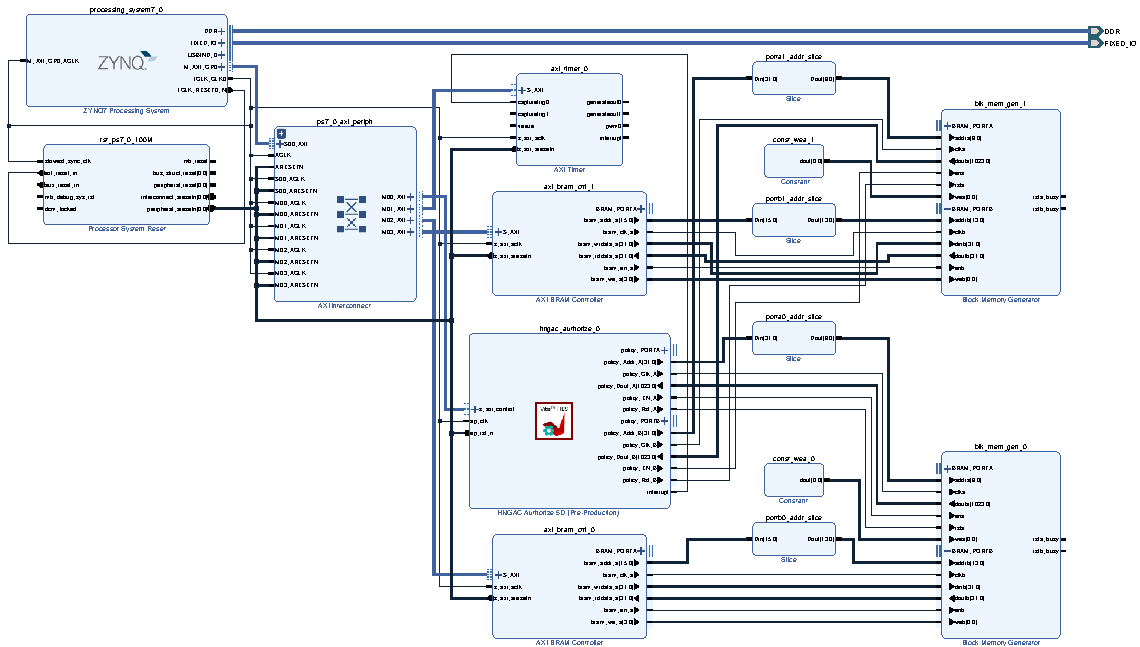
\includegraphics[width=\textwidth]{fig-system-bd.pdf}
\caption{\new{Vivado block design of the measured system on the PYNQ-Z1. The five-dimensional kernel (\texttt{hngac\_authorize\_0}, centre) reads policy from dual-port block RAM through two AXI BRAM controllers and receives requests from the Zynq processing system over the AXI interconnect. The AXI Timer (upper centre) latches the decision interval in hardware and is the source of the board cycle counts in Table~\ref{tab:board}.}}
\label{fig:systembd}
\end{figure*}

Determinism is structural, not observed. The scan executes $\lceil n/2 \rceil + 1$ pipeline iterations regardless of where, or whether, a match occurs. A permit latches the decision but does not shorten the scan, and an odd rule count pads with an all-zero rule that cannot match. Thus minimum, mean and maximum latency are equal by construction, and the measured closed form
\begin{equation}
L(n) = 12 + n/2 \ \text{cycles}
\label{eq:latency}
\end{equation}
holds exactly at every policy size we tested, where the constant 12 covers interface handshake and pipeline fill. At 100~MHz, $L(500) = 262$ cycles is 2.62~$\mu$s, and the 512-rule capacity bounds the primitive at 2.68~$\mu$s. A designer needing a tighter bound shrinks $n$ or raises the clock. Either way the bound is known before deployment, which is what makes the worst case a synthesis parameter.

Forgoing early exit costs the average case. A software scan that exits on first match beats \eqref{eq:latency} whenever the match lands early. We spend the average case to buy a worst case with zero variance, because a control loop budgets against the worst case.

\section{Experimental Method}
\label{sec:method}

\subsection{Platforms}

Hardware results come from Vitis HLS 2025.2 targeting the Zynq-7020 (xc7z020-clg400-1, the PYNQ-Z1 part) at a 10~ns clock. \new{Three kernels were synthesized and co-simulated: three-dimensional checking the identity triple, four-dimensional adding runtime state, and five-dimensional adding command provenance. They differ only in the conjunction terms of the rule check. Policy layout, pipeline structure, interface and testbench are common.} Cycle counts are taken from Verilog co-simulation transaction reports, which are cycle accurate\new{, and are corroborated on PYNQ-Z1 silicon by an AXI Timer that latches the decision interval in hardware}. Functional correctness is verified on the same silicon. Software results come from an Intel i7-12800H running the same kernel code compiled with g++ -O3, measured with Linux perf over 200{,}000 iterations after 1{,}000 warmup iterations per model. The ROS~2 evaluation runs on ROS~2 Jazzy.

\subsection{Request corpus}

For each policy rule the generator emits one request that satisfies all five dimensions, plus a state-failing and a provenance-failing variant where applicable. That yields eleven requests at four rules and 1{,}334 at 500, or 2{,}307 across all six sizes. The corpus exercises permits, state denials and provenance denials at every policy size, and the correctness columns of Section~\ref{sec:results} are computed on it. \new{RTL results use this corpus, sized to co-simulation runtime. The software comparison of Section~\ref{sec:results} instead replays a request mix over 200{,}000 iterations, so its denominators are decision counts rather than distinct requests.}

\subsection{Honesty rules}

We label every number by how it was obtained. Hardware cycle counts are measured and deterministic, and no confidence interval applies because variance is zero by construction. Software per-decision cycle counts are derived, not counter reads: perf supplies a measured effective clock of 4.96~GHz, and cycles are mean nanoseconds times that clock. Proportions from the adversarial run carry exact denominators and one-sided 95\% Wilson bounds. One baseline, RBAC with a modeled external state lookup, is a synthetic busy-wait, and we exclude it from every empirical claim in favor of the measured SQLite variant. The timing-window measurement produced zero slips and is reported only as a null result. \new{Board cycle counts are hardware-latched by an AXI Timer and are measurements. Board round-trip latency includes the Linux userspace stack on the processing system and is reported as an observation of that stack, never as a property of the kernel.}

\section{Results}
\label{sec:results}

\subsection{The key finding: dimensionality is free in time}

Table~\ref{tab:cycles} reports co-simulated kernel cycles per decision. The \new{three-, }four- and five-dimensional kernels resolve in an identical number of cycles at every policy size, with identical initiation interval, \new{an identical 6.965~ns estimated clock against the 10.00~ns target, }and identical 0.33~ns timing slack. Minimum, mean and maximum are equal at every point\new{, all three co-simulations pass,} and the closed form \eqref{eq:latency} fits all \new{eighteen} points exactly. \new{Adding the state dimension to the identity triple costs zero clock cycles, and adding provenance on top of state costs zero more.}

\begin{table}[t]
\caption{Kernel cycles per decision (Verilog co-simulation). Min, mean and max are equal at every point, and the \new{three} variants are identical columns.}
\label{tab:cycles}
\centering
\begin{tabular}{rrrrr}
\toprule
Rules & Requests & \new{3D cycles} & 4D cycles & 5D cycles \\
\midrule
4 & 11 & \new{14} & 14 & 14 \\
10 & 27 & \new{17} & 17 & 17 \\
50 & 134 & \new{37} & 37 & 37 \\
100 & 267 & \new{62} & 62 & 62 \\
200 & 534 & \new{112} & 112 & 112 \\
500 & 1{,}334 & \new{262} & 262 & 262 \\
\bottomrule
\end{tabular}
\end{table}

\new{One row of Table~\ref{tab:resources} is not identical. Iteration latency is two cycles in three dimensions and three in four and five, so pipeline depth grows by one stage when state arrives and then stops when provenance is added. Because the initiation interval is one, that depth is amortized across the scan and never reaches the per-decision cycle count. That is why Table~\ref{tab:cycles} is flat while pipeline depth is not. Dimensionality is absorbed into the width of a pipeline stage, not the length of the pipeline, until a stage runs out of timing slack.}

\new{Dimensionality} is not free in area. Table~\ref{tab:resources} \new{prices it. The fourth dimension costs 812 LUTs (+21.6\%) over the identity triple and the fifth a further 524 (+11.4\%), so carrying both costs 1{,}336 LUTs (+35.5\%) and 331 flip-flops (+14.1\%). All three kernels use zero BRAM and zero DSP. The five-dimensional kernel occupies 9\% of the part against the three-dimensional kernel's 7\%, so two added dimensions cost about two percentage points of a \$100 device.} An earlier four-dimensional build completed Vivado place and route with +2.170~ns worst negative slack and zero failing endpoints of 1{,}987, so the co-simulated clock is not optimistic for this fabric.

\begin{table}[t]
\caption{Resource utilization from synthesis (Zynq-7020, 100 MHz). \new{Percentages are of the available part resource.}}
\label{tab:resources}
\centering
\begin{tabular}{lrrr}
\toprule
Metric & \new{3D} & 4D & 5D \\
\midrule
II & \new{1} & 1 & 1 \\
Iteration latency & \new{2} & 3 & 3 \\
LUT & \new{3{,}768 (7\%)} & 4{,}580 (8\%) & 5{,}104 (9\%) \\
FF & \new{2{,}348 (2\%)} & 2{,}579 (2\%) & 2{,}679 (2\%) \\
BRAM & \new{0} & 0 & 0 \\
DSP & \new{0} & 0 & 0 \\
\new{Est. clock} & \new{6.965 ns} & \new{6.965 ns} & \new{6.965 ns} \\
Timing slack & \new{0.33 ns} & 0.33 ns & 0.33 ns \\
\bottomrule
\end{tabular}
\end{table}

\subsection{\new{Identical cycles, different security}}

\new{Table~\ref{tab:cycles} shows three kernels spending the same cycles. Table~\ref{tab:rtlauth} shows them answering different questions. We ran the identical 2{,}307-request corpus through all three co-simulations, so these are RTL decisions, not software model decisions.}

\begin{table}[t]
\caption{\new{Requests permitted per dimensional variant, same corpus, same co-simulation, identical cycle cost. The corpus supplies one satisfying request per rule plus state-failing and provenance-failing variants whose identity triple is valid.}}
\label{tab:rtlauth}
\centering
\newcolor
\begin{tabular}{rrrrr}
\toprule
Rules & Requests & 3D permits & 4D permits & 5D permits \\
\midrule
4 & 11 & 11 & 8 & 4 \\
10 & 27 & 27 & 19 & 10 \\
50 & 134 & 134 & 92 & 50 \\
100 & 267 & 267 & 184 & 100 \\
200 & 534 & 534 & 367 & 200 \\
500 & 1{,}334 & 1{,}334 & 917 & 500 \\
\midrule
Total & 2{,}307 & 2{,}307 & 1{,}587 & 864 \\
\bottomrule
\end{tabular}
\end{table}

\new{The three-dimensional kernel permits the entire corpus, all 2{,}307 requests, at every policy size. This is not a defect. Every request carries a valid identity triple and the variants differ only in the state and provenance fields, so a kernel that cannot represent $\sigma$ or $\pi$ has no basis to deny any of them. It answers its own question correctly. That question is not the one Layla's interlock asks.}

\new{The four-dimensional kernel denies the state-failing variants and admits the provenance-failing ones, permitting 1{,}587. The five-dimensional kernel permits 864, exactly one satisfying request per rule at each policy size. Across the total row, 1{,}443 requests separate three dimensions from five, and 723 of those separate four from five. Each gap is an attack class: unsafe-state operation (CVE-2022-33323) and command provenance abuse (CVE-2021-38425).}

\new{The two tables move independently. The cycle columns are identical and the permit columns are not. In hardware, the security question a kernel can ask is decoupled from what asking it costs in time.}

\subsection{In software, the same dimension is not free}

The same kernel logic compiled for the i7 and measured under perf tells the opposite story. Per-rule marginal cost rises from 0.645 cycles in three dimensions to 1.024 in four and 1.220 in five, \new{a 19\% increase for the fifth dimension alone}. In software every rule pays for every dimension on every decision, and the cost compounds with policy size. At 500 rules the five-dimensional software path spends 685 derived cycles per decision against the hardware kernel's 262 measured cycles. Figure~\ref{fig:keyfinding} plots both families. The software curves fan out as dimensions are added\new{, and the three hardware curves are one line}.

\begin{figure}[t]
\centering
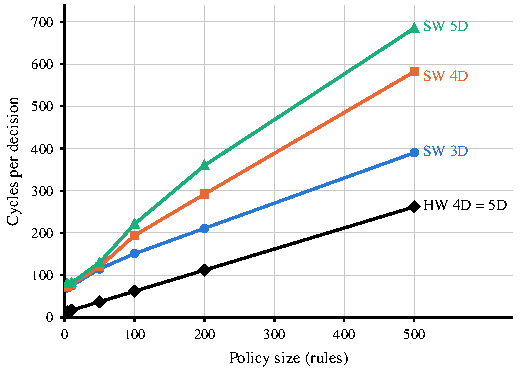
\includegraphics[width=\columnwidth]{fig-key-finding.pdf}
\caption{Cycles per decision versus policy size. Software cycles are derived from perf-measured means and the 4.96~GHz clock; hardware cycles are co-simulated. Software slopes steepen with each added dimension. \new{The 3D, 4D and 5D hardware series are identical at every measured point and render as one line.}}
\label{fig:keyfinding}
\end{figure}

\subsection{Faster baselines are faster because they are wrong}

Table~\ref{tab:models} compares six software models over 200{,}000 replayed decisions. The RBAC hash map resolves in roughly 100 derived cycles at every policy size, and that flat cost is genuine. It also admits 200{,}000 of 200{,}000 decisions, including all 100{,}000 that violate state, and the DAG-NGAC and three-dimensional paths admit the same. A model that cannot see state or provenance cannot deny on them. The only software models that decide correctly are the five-dimensional path and a flattened direct-lookup table that buys its speed with 19.7$\times$ the memory. An RBAC deployment could encode state into its roles, a maintenance operator distinct from a normal operator, but sixteen state bits and three source types multiply that role count combinatorially. The alternative, RBAC consulting an external state store, cost 20.6 times the four-dimensional path against an in-process SQLite store. Table~\ref{tab:models} is not an argument that cheap static authorization suffices. The fast rows are fast because they answer a smaller question than the one Layla's interlock asks.

\begin{table}[t]
\caption{Software models, derived cycles per decision at 500 rules, and correctness over the replayed request mix. ``Over'' = admits state- or provenance-violating requests.}
\label{tab:models}
\centering
\begin{tabular}{lrl}
\toprule
Model & Cycles (500) & Decides correctly? \\
\midrule
H-NGAC 3D & 390 & No, over-authorizes \\
H-NGAC 4D & 582 & No, over-authorizes \\
H-NGAC 5D & 685 & \textbf{Yes} \\
RBAC hash map & 100 & No, over-authorizes \\
DAG-NGAC traversal & 1{,}032 & No, over-authorizes \\
Flattened 5D lookup & 984 & \textbf{Yes}, 19.7$\times$ memory \\
\bottomrule
\end{tabular}
\end{table}

\subsection{Adversarial evaluation in ROS 2}

We ran the provenance-abuse scenario live. A software gatekeeper node running the same five-dimensional decision function fronted an actuator topic while a legitimate node and a compromised node both published with valid credentials for the same subject, the compromised node at five times the legitimate rate. Over a 30-second session the policy blocked 18{,}878 of 18{,}878 injection attempts, a 100\% block rate with a one-sided 95\% Wilson lower bound of 99.99\%, and passed 17{,}059 of 17{,}059 legitimate commands, a 0\% false positive rate with a 95\% upper bound of 0.02\%. This run and the silicon run carry separate claims. The first establishes what the five-dimensional semantics block under sustained adversarial load, the second that the synthesized kernel reproduces those decisions on all 2{,}307 corpus requests. Under three- or four-dimensional policy every injection would have been admitted, because the attacker's identity triple and state context were valid. Only provenance separates the two streams.

The same runs measured the timing window. Under idle and saturated CPU load, zero of 8{,}733 authorization callbacks exceeded the 50~$\mu$s lower bound of DDS localhost propagation. We report this as a null result. The argument stands on \eqref{eq:latency}: a synthesis-time bound below the propagation floor closes the window by construction, which no software mean can do.

\subsection{\new{On silicon}}
\label{subsec:onsilicon}

\new{Co-simulation is cycle accurate but still simulation. We placed the five-dimensional kernel on a PYNQ-Z1 at 100~MHz behind an AXI Timer and read the decision interval from a hardware-latched counter. Table~\ref{tab:board} reports it against the co-simulated counts.}

\begin{table}[t]
\caption{\new{On-board AXI Timer capture (PYNQ-Z1, 100 MHz, full corpus) against co-simulated kernel cycles. Board minimum, mean and maximum are equal at every policy size.}}
\label{tab:board}
\centering
\newcolor
\begin{tabular}{rrrr}
\toprule
Rules & Co-sim cycles & Board cycles & Offset \\
\midrule
4 & 14 & 39 & 25 \\
10 & 17 & 42 & 25 \\
50 & 37 & 62 & 25 \\
100 & 62 & 87 & 25 \\
200 & 112 & 137 & 25 \\
500 & 262 & 287 & 25 \\
\bottomrule
\end{tabular}
\end{table}

\new{The board tracks co-simulation with a constant 25-cycle offset at all six policy sizes, and minimum, mean and maximum are equal on silicon as they are in simulation. The offset is the AXI-Lite handshake that moves the request in and the decision out. Being constant, it enters \eqref{eq:latency} as an additive term rather than a source of variance. The determinism argued from pipeline structure in Section~\ref{sec:arch} holds on the real part.}

\new{The same run measured round-trip latency from the processing system, and that number behaves differently. Mean round trip rises from 2.09~$\mu$s at four rules to 4.77~$\mu$s at 500, but the maximum reaches 5.92~ms at 500 rules, three orders of magnitude above its own mean. The tail comes entirely from the Linux userspace stack on the board's Cortex-A9 between the timer read and the application, the same mechanism behind the i7's tail in Section~\ref{subsec:comparison}. A deterministic primitive does not make a non-deterministic caller deterministic. It bounds the part of the path a designer can bound, and Table~\ref{tab:board} is that part.}

\subsection{Mean versus worst case}
\label{subsec:comparison}

The fabric does not outpace the CPU, and we say so directly. At 500 rules the i7 completes a mean five-dimensional decision in 138~ns of wall clock against the fabric's 2.62~$\mu$s, because a 4.96~GHz core is 49.6 times faster per cycle than a 100~MHz fabric. The CPU wins the mean by roughly 19$\times$. The defensible comparison is the worst case, and there the ordering reverses. The software path's worst observed decision at 200 rules was 355.4~$\mu$s against the fabric's invariant 1.12~$\mu$s, and its worst at four rules was 298.8~$\mu$s against 0.14~$\mu$s. Further, the software figure is an observation, not a bound: the 157~$\mu$s outlier in the DCAS baseline arrived in a run whose mean was 1.14~$\mu$s \cite{karim2026dcas}. An operating system does not guarantee its own tail, and a control loop budgets for the tail. Figure~\ref{fig:tail} plots both. The software mean runs below the hardware bound at every policy size and the worst case runs above it at every size, by more than three orders of magnitude at four rules. The worst case does not track policy size, because the tail belongs to the scheduler and not to the policy.

\begin{figure}[t]
\centering
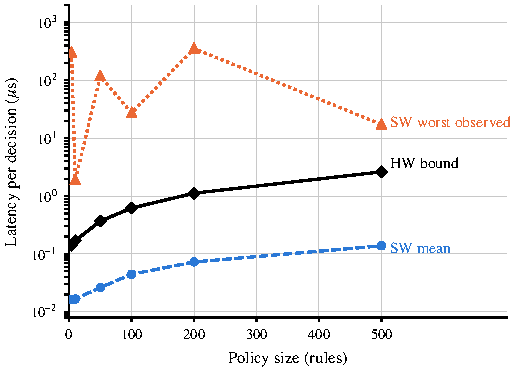
\includegraphics[width=\columnwidth]{fig-tail.pdf}
\caption{Wall-clock latency per decision, log scale. The software mean and worst observed come from perf measurements of the five-dimensional path. The hardware line is the closed-form bound of \eqref{eq:latency} at 100~MHz, where minimum, mean and maximum coincide. The software worst case is an observation, not a bound, and does not track policy size.}
\label{fig:tail}
\end{figure}

% AUTHOR DECISION: OPA/XACML reuse from TS-NGAC (approved for manuscript per
% canonical-context, flagged as open in manuscript-agent-prompt rule 8).
% Cut this paragraph if the journal contribution split argues otherwise.
General-purpose policy engines sit on the same axis. In an earlier evaluation, Open Policy Agent averaged 271.491~$\mu$s per decision with 13 deadline misses \cite{karim2026tsngac}, and an XACML OpenPDP deployment averaged roughly 50~ms \cite{karim2026dcas, oasisxacml}. These engines evaluate far richer policy than \eqref{eq:match} expresses. They also occupy a latency regime three to five orders of magnitude above \eqref{eq:latency}, the regime that keeps authorization out of control paths.

\section{Limitations}
\label{sec:limitations}

\new{First, the parity result covers three, four and five dimensions on one part at one clock. We have not shown that an arbitrary sixth dimension is free, only that these two were, and Section~\ref{sec:arch} names the mechanism that would end the pattern.} \new{Second,} the software baseline is a 4.96~GHz laptop CPU while the fabric runs at 100~MHz. A baseline on the board's own Cortex-A9 would make the wall-clock comparison fairer, and we did not run it. \new{The board data bounds the fabric and the interface, not a software decision path on the same silicon.} \new{Third,} software latency distributions were measured under WSL2, whose scheduler jitter contaminates maxima, which is why we cite worst observed values and never call them WCETs. \new{Fourth,} the primitive is capacity-bounded at 512 rules and 256 policy nodes, and policy update happens off the decision path. \new{Fifth,} the modeled external-state lookup is synthetic and excluded from every empirical claim, since the measured SQLite path shows the same thing. \new{Sixth,} the kernel compiles only the association subset of INCITS 565, so no claim extends beyond rules that grant. \new{Seventh,} the zero-cycle result holds at one operating point, 100~MHz on a Zynq-7020, where \new{all three} kernels close timing with +0.33~ns slack. At an aggressive clock target \new{an} added dimension could force another pipeline stage, the boundary the hypothesis of Section~\ref{sec:model} predicts\new{. The two-to-three step in iteration latency already shows that mechanism operating below the threshold where it costs cycles}. Characterizing the frequency ceiling is future work.

\section{Future Work and Conclusion}
\label{sec:conclusion}

Four questions follow. \new{1.~At what clock does the next dimension stop being free, and does that ceiling move with policy width or only with stage depth? 2.~What does a software decision path on the board's own Cortex-A9 cost, so the wall-clock comparison runs at one class of silicon?} 3.~Does \eqref{eq:latency} survive a dynamic policy update path, or does update traffic reintroduce jitter? 4.~How does the primitive compose with time-scoped delegation, which TS-NGAC develops in software \cite{karim2026tsngac}? Further, we call on the community to report authorization performance as cycle-level worst cases rather than means, because a mean is the statistic a control loop cannot budget against.

We extended the H-NGAC bitmask primitive with system-state and command-provenance dimensions and synthesized \new{three-, }four- and five-dimensional kernels to a Zynq-7020. The added \new{dimensions} cost zero clock cycles and \new{1{,}336} LUTs. Latency is closed-form at $12 + n/2$ cycles with zero jitter by construction\new{, confirmed on silicon by a hardware-latched counter. At identical cycle cost, the three-dimensional kernel permits in full the same corpus the five-dimensional kernel denies 1{,}443 times}, and the five-dimensional policy blocked 18{,}878 of 18{,}878 credentialed injection attempts in ROS~2 with zero false positives in 17{,}059 legitimate commands. Robotics and functional-safety engineers can treat the authorization worst case as a synthesis parameter, place the decision inside the control loop budget, and close the two attack classes identity-based authorization admits. Layla's interlock becomes a policy bit the fabric checks in bounded time, not a procedure she hopes the operator follows.

\bibliographystyle{IEEEtran}
\bibliography{refs}

\end{document}
